\section{Architettura}
	Il nostro prodotto è composto da un plug-in sviluppato per la piattaforma Grafana e un'applicazione esterna a quest'ultima. L'analisi dell'architettura sarà quindi divisa per questi due componenti.
	\subsection{Plug-in interno a Grafana}
		Per poter apprezzare la suddivisione del prodotto viene riportato il diagramma dei Package, allegato nel file plug-in-package.png, che rappresenta le dipendenze definite ad alto livello tra le componenti.
		\subsubsection{Progettazione architetturale}
		Per la progettazione architetturale del plug-in si è deciso di utilizzare il design pattern MVC. Abbiamo preso questa decisione perché si adatta bene allo sviluppo di software all'interno della piattaforma Grafana. In particolare è così strutturata:
		\begin{itemize}
			\item \textbf{Model}: all'interno del Model gestiamo la business logic del nostro prodotto, più in dettaglio la predizione dei dati sulla base degli algoritmi che abbiamo implementato, la lettura dei dati da utilizzare e la scrittura dell'esito della loro elaborazione tramite un database Influx, considerato lo standard per la piattaforma Grafana;
			\item \textbf{View}: all'interno della View gestiamo la presentation logic del nostro prodotto, più in dettaglio la creazione di un pannello della dashboard di Grafana e le sue interazioni con l'utente;
			\item \textbf{Controller}: all'interno del Controller gestiamo l'application logic del nostro prodotto, più in dettaglio la necessaria trasformazione dei dati forniti dall'utente in un formato utilizzabile dai componenti del Model.
		\end{itemize}
		In allegato forniamo il diagramma delle classi nel file plug-in-diagramma-classi.png .
		\subsubsection{Progettazione di dettaglio}
			\paragraph{Model}
			Come prima cosa all'interno del modello abbiamo inserito gli algoritmi di predizione. Per la progettazione dei componenti che li implementano, abbiamo deciso di privilegiare l'estensibilità creando un'interfaccia \textit{AlgorithmPrediction} che da contratto fornisce il metodo \textit{predict(dataset, configuration, influxParams)} che riceve in input i dati e la configurazione per eseguire l'algoritmo e i parametri per connettersi e salvare il risultato su InfluxDB.
			In questo modo è possibile implementare nuovi algoritmi a partire dalla suddetta interfaccia, rispettando i parametri espressi. Noi abbiamo implementato gli algoritmi Support Vector Machine e Regressione lineare e quindi abbiamo fornito due implementazioni concrete dell'interfaccia.
			\textit{SvmPrediction} è la classe che implementa l'algoritmo SVM ed importa la libreria ml-modules mentre \textit{RlPrediction} è quella che implementa RL ed importa LinearRegression dalla libreria \textit{regression.module}. Entrambe sono caratterizzate da un campo dati writeInflux che rappresenta un oggetto di Classe WriteInflux che viene quindi istanziato nel costruttore. Questo rappresenta una dipendenza di tipo composizione e risulta essere esplicita. 
			Infine la classe concreta \textit{WriteInflux} che importa la libreria \textit{node-influx} rappresenta la connessione con il database influxDB e di conseguenza una dipendenza con esso. In questo caso non si è scelto di fornire un'interfaccia in quanto all'intero di Grafana viene utilizzato questo db come standard. Presenta due metodi per la scrittura sul database rispettivamente \textit{WriteArrayToInflux(data, timeStamp)} che permette di scrivere i dati e \textit{writeStampsToInflux(point, timeStamp)} che permette di inserire il timeStamp, caratteristico di un database TimeScale come Influx. 
			\mbox{}
			\begin{landscape}
				\begin{figure}
					\begin{figure} [H]
						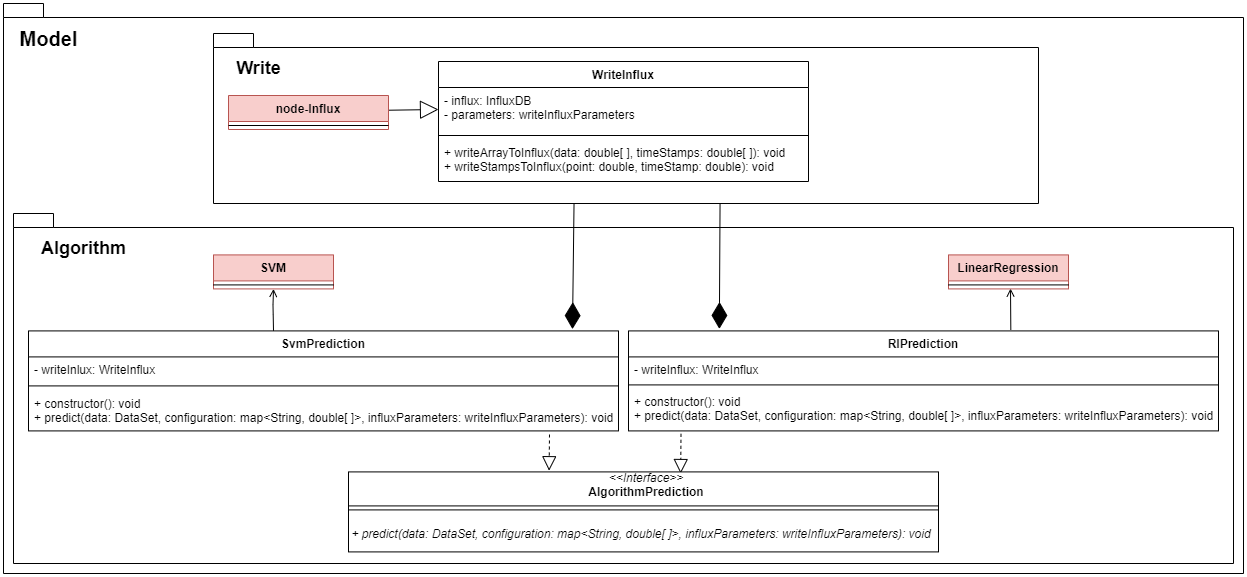
\includegraphics[width=\linewidth]{./img/Diagrammi/d1.png}
						\caption{Diagramma delle classi del Model}
					\end{figure}
				\end{figure}
			\end{landscape}
			Per la comunicazione dei dati tra Model e View ci appoggiamo al funzionamento di Grafana che la implementata utilizzando un design pattern Observer. 
			\paragraph{View}
			All'interno della vista abbiamo inserito la componente Panel rappresentata dalla classe \textit{PanelCtrl} che estende la classe \textit{MetricsPanelCtrl} di Angular. Essa permette la visualizzazione dei risultati delle query su Influx.
			Inoltre è presente la classe \textit{SelectInfluxDBCtrl} che rappresenta la componente di ricezione della datasource definita e connessa dall'utente tramite l'interfaccia grafica. Essa è in relazione di composizione con \textit{PanelCtrl} che la contiene e ne gestisce il ciclo di vita; infatti non ha senso di esistere al di fuori del pannello che permette la visualizzazione dei dati che legge.
			Per implementare i grafici, invece, abbiamo deciso di utilizzare un componente della libreria Plotly che importiamo e gestiamo internamente dentro \textit{PanelCtrl}.
			Infine nella classe \textit{PanelCtrl} è presente un campo dati che rappresenta un oggetto di tipo ProcessData che viene gestito interamente. Perciò è presente una dipendenza di composizione tra queste due classi che definisce anche la relazione che sussiste tra View e Model del nostro prodotto. 
			\mbox{}
			\begin{landscape}
			\begin{figure} [H]
				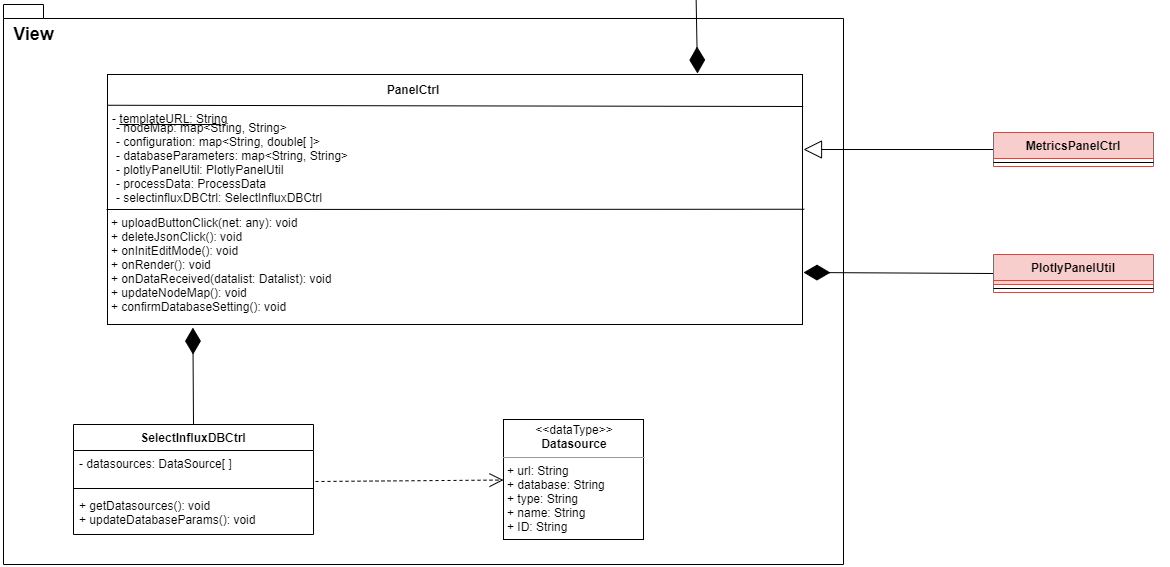
\includegraphics[width=\linewidth]{./img/Diagrammi/d2.png}
				\caption{Diagramma delle classi della View}
			\end{figure}
		\end{landscape}
			\paragraph{Controller}
			All'interno del controller viene implementata la mappatura tra i dati e le richieste ricevute dalla View e le chiamate alla business logic per la loro esecuzione. Abbiamo deciso di implementare un design pattern strategy ottenendo la seguente struttura:
			\begin{itemize}
				\item \textbf{ProcessData}: questa è una classe concreta che rappresenta il context e al suo interno viene scelto, sulla base dei dati e della richieste ricevute, quale strategia seguire, che in questo caso è rappresentata da quale algoritmo di predizione processare;
				\item \textbf{PerformPrediction}: questa è un'interfaccia che rappresenta la strategia astratta. Essa definisce il contratto che un componente che processa i dati per un determinato algoritmo deve avere per essere tale;
				\item \textbf{ProcessSvm}: questa è una classe concreta che implementa \textit{PerformPrediction} e rappresenta il componente che esegue la mappatura e il controllo dei dati per fornirli all'algoritmo di predizione Svm;
				\item \textbf{ProcessRl}: questa è una classe concreta che implementa \textit{PerformPrediction} e rappresenta il componente che esegue la mappatura e il controllo dei dati per fornirli all'algoritmo di predizione Rl.
			\end{itemize}
			All'interno di \textit{ProcessSvm} e \textit{ProcessRl} è presente un attributo rispettivamente SvmPredicter e RlPredicter che definisce una dipendenza di tipo composizione e di conseguenza il collegamento tra Controller e Model.
			\mbox{}
			\begin{landscape}
			\begin{figure} [H]
				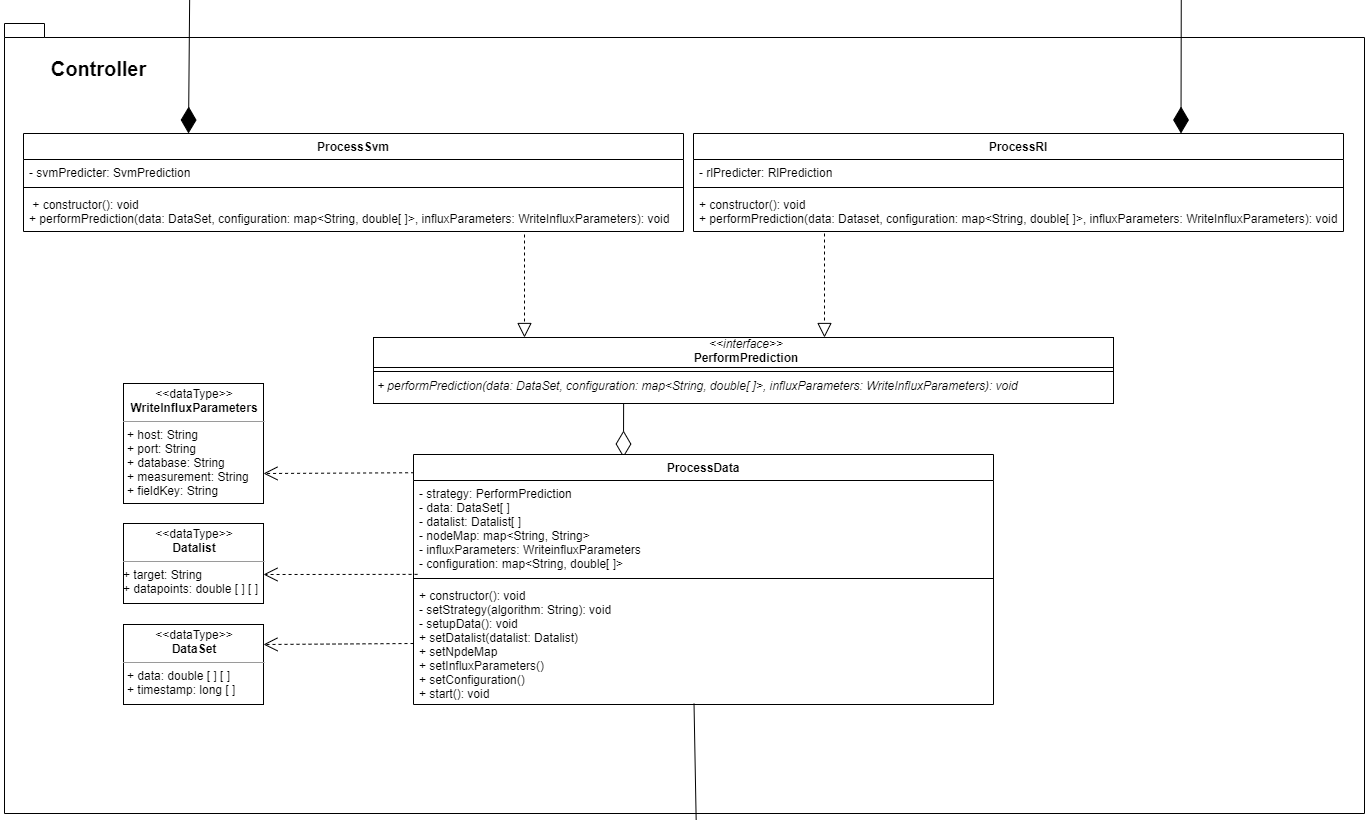
\includegraphics[width=\linewidth]{./img/Diagrammi/d3.png}
				\caption{Diagramma delle classi del Controller}
			\end{figure}
		\end{landscape}
	\subsection{Applicazione esterna alla piattaforma Grafana}
	Per poter apprezzare la suddivisione del prodotto viene riportato il diagramma dei Package, allegato nel file app-package.png, che rappresenta le dipendenze definite ad alto livello tra le componenti.
		\subsubsection{Progettazione architetturale}
			Per la progettazione architetturale dell'applicazione esterna a Grafana si è deciso di utilizzare il design pattern MVVM. Abbiamo preso questa decisione perché si adatta molto bene alle tecnologie che utilizziamo ovvero React ed Electron. In particolare è così strutturata:
		\begin{itemize}
			\item \textbf{Model}: all'interno del Model gestiamo la business logic dell'applicazione, più in dettaglio eseguiamo l'addestramento dei dati attraverso gli algoritmi di predizione e le operazioni di input-output attraverso i file;
			\item \textbf{View}: all'interno della View gestiamo la presentazione dei dati attraverso React;
			\item \textbf{ViewModel}: all'interno del ViewModel implementiamo il binding tra la vista ed il modello. Più in dettaglio il binding tra View e ViewModel ci viene fornito da Electron mentre quello tra Model e ViewModel viene implementato tramite l'utilizzo delle callback.
		\end{itemize}
		In allegato forniamo il diagramma delle classi nel file app-diagramma-classi.png.
		\subsubsection{Progettazione di dettaglio}
			\paragraph{Model}
			Progettando il modello dell'applicazione esterna abbiamo riscontrato la necessità di utilizzare in due diversi casi un Template Method: \\
			\textbf{Read} \mbox{} \\ 
			Abbiamo notato che nella gestione dell'input, indipendentemente dall'estensione del file ricevuto, l'algoritmo per eseguire la lettura di quest'ultimo aveva uno scheletro comune. È stato quindi deciso di implementare un template method. La classe astratta Read implementa il metodo readFile(path, callback) che definisce l'algoritmo comune, esegue una lettura dal file system del file e chiama una funzione parser(data, callback) che viene implementata nelle classi concrete ReadCsv e ReadJson a seconda delle specifiche esigenze dell'estensione del file. La funzione readFile(path, callback) restituisce infine una stringa, mediante la chiamata della callback, contenente le informazioni lette. 
			\mbox{}
			\begin{figure} [H]
				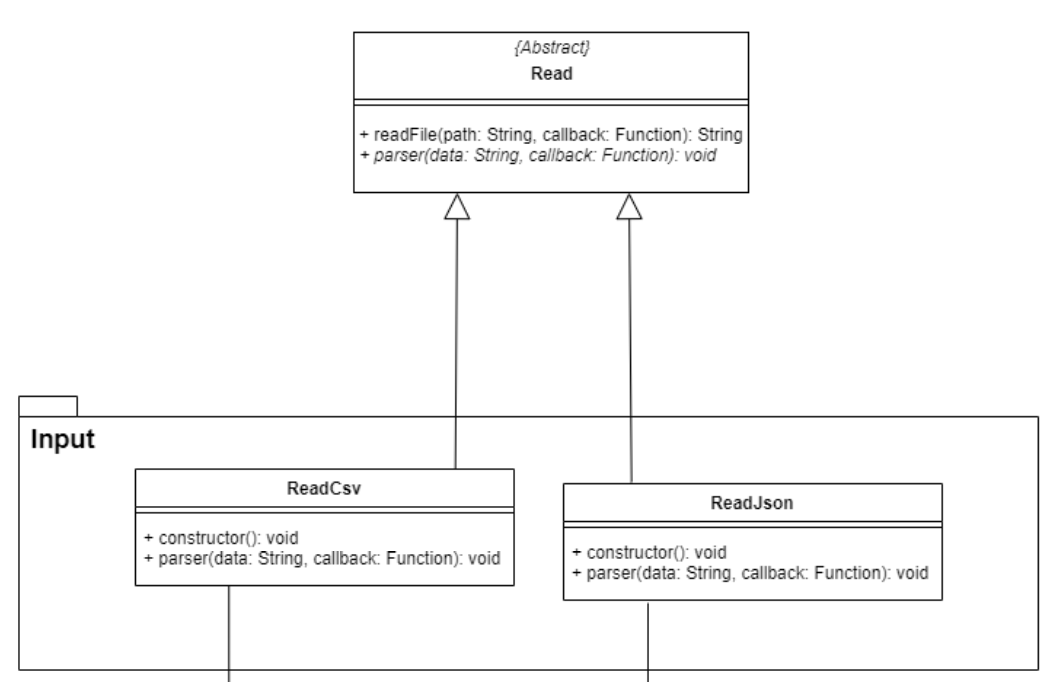
\includegraphics[width=\linewidth]{./img/Diagrammi/Read.png}
				\caption{Diagramma delle classi del Template Method Read}
			\end{figure}
			\textbf{Write} \mbox{} \\ 
			Progettando la gestione degli output ci si è accorti che indipendentemente dall'estensione del file da scrivere, l'algoritmo di scrittura aveva uno scheletro comune. È stato quindi deciso di implementare un template method per eventuali sviluppi futuri. La classe astratta Write implementa il metodo writeToDisk(path, name, data, notes, callback) che definisce l'algoritmo comune. Viene chiamata la funzione buildTrainedFile(result, notes), implementata nella classe concreta WriteJson, che restituisce una map<String, double> che rappresenta l'oggetto da scrivere nel file da dare in output. Viene poi chiamata la funzione parser(data, callback), implementata nella classe concreta WriteJson, che trasforma questo oggetto in una stringa. Il metodo writeToDisk(path, name, data, notes, callback) riceverà infine questa stringa tramite la callback e la scriverà in un file da dare in output.
			\mbox{}
			\begin{figure} [H]
				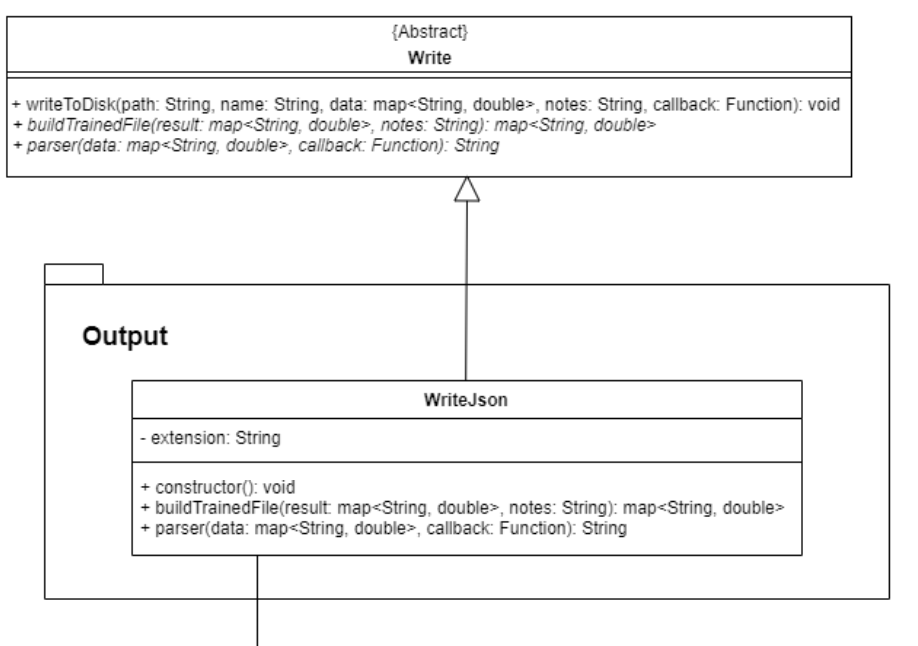
\includegraphics[width=\linewidth]{./img/Diagrammi/write.png}
				\caption{Diagramma delle classi del Template Method Write}
			\end{figure}
			Inoltre abbiamo implementato gli algoritmi di predizione attraverso un'interfaccia \textit{AlgorithmTrainer}. Essa permette l'estensibilità a qualunque algoritmo purché rispetti il contratto definito. Attualmente abbiamo implementato \textit{SvmTrainer} e \textit{RlTrainer} ovvero le classi rispettivamente dell'addestramento di Svm ed Rl.
			Per le funzionalità sopra elencate, implementiamo l'invio delle notifiche alla ViewModel per l'aggiornamento dei dati tramite il meccanismo di callback.
			\mbox{}
			\begin{landscape}
			\begin{figure} [H]
				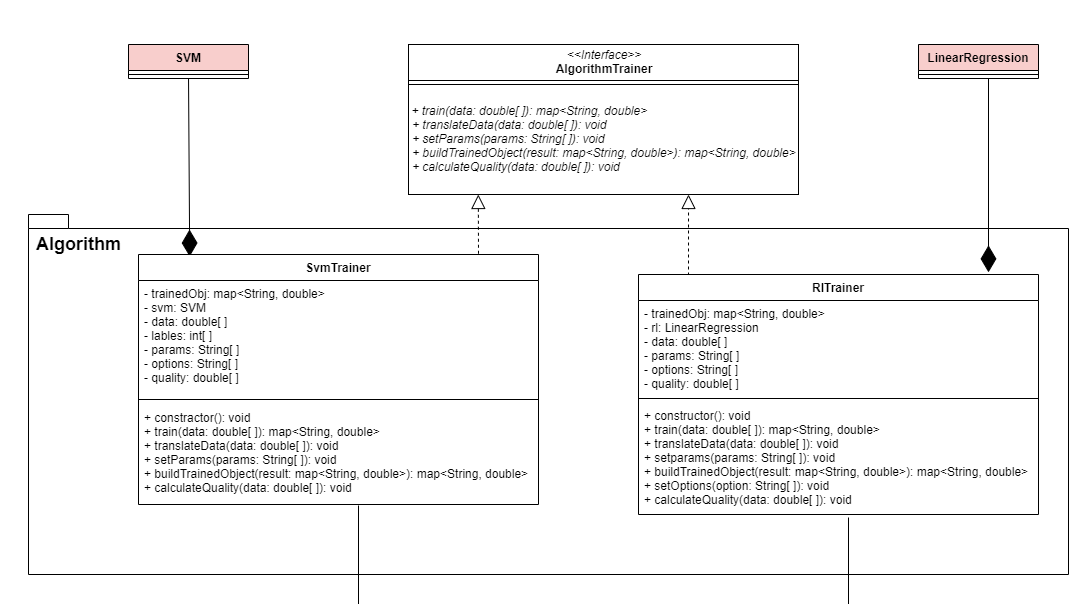
\includegraphics[width=\linewidth]{./img/Diagrammi/Training.png}
				\caption{Diagramma delle classi di Training}
			\end{figure}	
			\end{landscape}		
			\paragraph{View}
			La parte di presentazione dei dati verso l'utente è realizzata tramite dei componenti di React, contenuti nella classe principale App che li renderizza. Inoltre per la visualizzazione del grafico risultante dalla predizione abbiamo deciso di utilizzare la libreria D3. 
			La gestione dello stato dell'applicazione è delegata al ViewModel che si occupa di aggiornare lo stato che verrà poi renderizzato dalla vista. 	
			\paragraph{ViewModel}
			Nella parte di ViewModel dell'applicazione sono contenuti i dati da visualizzare nella vista e le operazioni che devono essere effettuate dal modello per soddisfare le richieste dell'utente. In particolare il ViewModel è legato alla vista tramite Electron che ne gestisce lo scambio di dati appoggiandosi al nostro componente EventManager e con il modello tramite il meccanismo di callback.
			Per il process dei dati abbiamo riscontrato la necessità implementare in tre diversi casi il design pattern strategy: \\
			\textbf{Reading} \mbox{} \\ 
			\begin{itemize}
				\item \textbf{ProcessReading}: questa è una classe concreta che rappresenta il context e al suo interno viene scelto, sulla base dei dati e della richieste ricevute, quale strategia seguire, che in questo caso è leggere un file Csv o un file Json;
				\item \textbf{PerformReading}: questa è un'interfaccia che rappresenta la strategia astratta. Essa definisce il contratto che un componente che legge un file in input deve avere per essere tale;
				\item \textbf{ProcessReadingCsv}: questa è una classe concreta che implementa \textit{PerformReading} e rappresenta il componente che esegue la lettura dei dati da un file Csv;
				\item \textbf{ProcessReadingJson}: questa è una classe concreta che implementa \textit{PerformReading} e rappresenta il componente che esegue la lettura dei dati da un file Json.
			\end{itemize}
			\mbox{}
			\begin{figure} [H]
				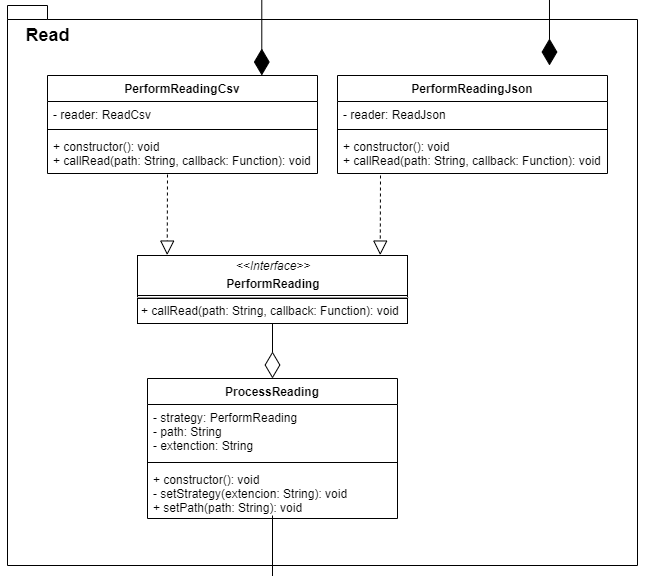
\includegraphics[width=\linewidth]{./img/Diagrammi/dAppR.png}
				\caption{Diagramma delle classi dello Strategy Reading}
			\end{figure}
			\textbf{Writing} \mbox{} \\ 
			\begin{itemize}
				\item \textbf{ProcessWriting}: questa è una classe concreta che rappresenta il context e al suo interno viene scelto, sulla base dei dati e della richieste ricevute, quale strategia seguire, che in questo caso è scrivere un file in base alla sua estensione;
				\item \textbf{PerformWriting}: questa è un'interfaccia che rappresenta la strategia astratta. Essa definisce il contratto che un componente che deve scrivere un file da dare in output deve avere per essere tale;
				\item \textbf{ProcessWritingJson}: questa è una classe concreta che implementa \textit{PerformWriting} e rappresenta il componente che esegue la scrittura dei dati su un file Json;
			\end{itemize}
			\mbox{}
			
				\begin{figure} [H]
					\begin{center}
					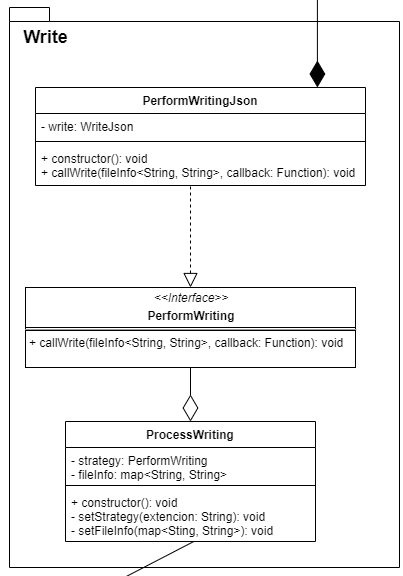
\includegraphics[width=90mm]{./img/Diagrammi/dAppW.png}
				\end{center}
					\caption{Diagramma delle classi dello Strategy Writing}
				\end{figure}
			
			\textbf{Training} \mbox{} \\ 
			\begin{itemize}
				\item \textbf{ProcessTraining}: questa è una classe concreta che rappresenta il context e al suo interno viene scelto, sulla base dei dati e della richieste ricevute, quale strategia seguire, che in questo caso è rappresentata da quale algoritmo di predizione addestrare;
				\item \textbf{PerformTraining}: questa è un'interfaccia che rappresenta la strategia astratta. Essa definisce il contratto che un componente che processa i dati per un determinato algoritmo deve avere per essere tale;
				\item \textbf{ProcessTrainingRl}: questa è una classe concreta che implementa \textit{PerformTraining} e rappresenta il componente che esegue la mappatura e il controllo dei dati per fornirli all'algoritmo di predizione Rl per eseguire il suo addestramento;
				\item \textbf{ProcessTrainingSvm}: questa è una classe concreta che implementa \textit{PerformTraining} e rappresenta il componente che esegue la mappatura e il controllo dei dati per fornirli all'algoritmo di predizione Svm per eseguire il suo addestramento.
			\end{itemize}
		\mbox{}			
			\begin{landscape}
			\begin{figure} [H]
				\begin{center}
					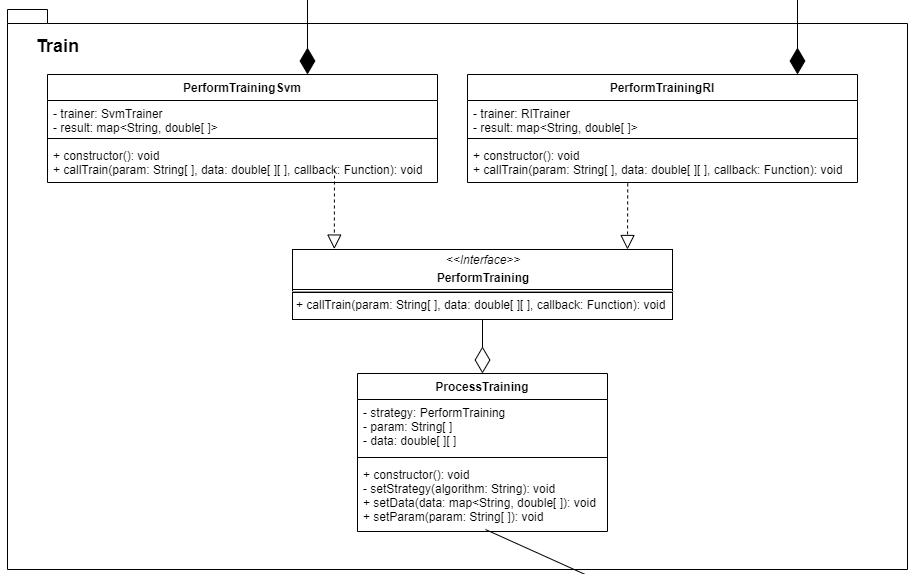
\includegraphics[width=350mm,height=110mm,keepaspectratio]{./img/Diagrammi/dAppT.png}
					\caption{Diagramma delle classi dello Strategy Training}
				\end{center}
			\end{figure}
			\end{landscape}